\newcommand{\mytoptext}{Πλήρης εξερεύνηση και κάλυψη αρχικά άγνωστου περιβάλλοντος με αυτόνομο, προσομοιωμένο όχημα}
\documentclass[12pt,a4paper,titlepage,oneside]{scrartcl}
% Argument 'table' for '\cellcolor{}' command.
% Should be high because it might get loaded by another package with different arguments:
% - http://tex.stackexchange.com/questions/87197/latex-error-option-clash-for-package-xcolor-for-table
% - http://tex.stackexchange.com/questions/83101/option-clash-for-package-xcolor
\usepackage[usenames, table]{xcolor}
% --------------------- FONTS & LANGUAGE ---------------------
\usepackage{amssymb,amsmath,amsthm,amsfonts}
%\usepackage{mathspec}
\usepackage[MnSymbol]{mathspec}
%\defaultfontfeatures{Mapping=tex-text}
\defaultfontfeatures{Scale=MatchLowercase,Numbers={Lining,Proportional}}

\setmainfont{MinionPro}[
    Path = fonts/,
    Extension = .otf,
    UprightFont = *-Regular,
    ItalicFont = *-Italic,
    BoldFont = *-SemiBold,
    BoldItalicFont = *-SemiBoldItalic
]
\setsansfont{MyriadPro}[
    Path = fonts/,
    Extension = .ttf,
    UprightFont = *-Regular,
    ItalicFont = *-Italic,
    BoldFont = *-SemiBold,
    BoldItalicFont = *-SemiBoldItalic
]
\setmathfont{xits-math.otf}
\setmathsfont[Set=Greek,Uppercase=Italic,Lowercase=Italic]{Minion Pro}
\setmonofont{inconsolatalgc}[
    Path = fonts/,
    Extension = .ttf,
    ItalicFont = *italic,
    BoldFont = *bold,
    BoldItalicFont = *bolditalic
]

% Polyglossia warning: due to a bug (https://github.com/reutenauer/polyglossia/issues/110) numbering with greek letters is incorrect.
% /usr/share/texmf-dist/tex/latex/polyglossia/gloss-greek.ldf must be edited.
% or \setmainlanguage[numerals=arabic]{greek} should be used instead.
\usepackage{polyglossia}
\setmainlanguage{greek}
\setotherlanguages{english}
\PolyglossiaSetup{greek}{indentfirst=true}
\PolyglossiaSetup{english}{indentfirst=true}

% ---------------------- MISCELLANEOUS PACKAGES ----------------------
% Minted package for the listings.
\usepackage[newfloat=true]{minted}
\setminted{%
    autogobble=true,%
    breaklines=true,%
    frame=single,%
    framerule=2pt,%
    linenos=false%
}
\setcounter{tocdepth}{3} % subsub has numbers
\setcounter{secnumdepth}{3} % subsub in toc

% For \includegraphics.
% https://ctan.org/pkg/graphicx
\usepackage{graphicx}
\graphicspath{{./figures/}{./images/}}

% Provides LaTeX the ability to create hyperlinks within the document.
% https://www.ctan.org/pkg/hyperref
% http://en.wikibooks.org/wiki/LaTeX/Hyperlinks#Hyperref
\usepackage{hyperref}
\hypersetup{
    colorlinks,
    linkcolor={blue!50!black},
    citecolor={blue!50!black},
    urlcolor={blue!70!black},
    breaklinks=true
}
% Make a hyperlink navigate to the top of the figure in LaTeX when using hyperref.
% http://stackoverflow.com/a/21251925/3430986
\usepackage{caption}
% Change the caption name for listing / code enviroment.
\captionsetup[listing]{name=Καταχώρηση}
% And list of listings.
% ftp://ftp.dante.de/tex-archive/macros/latex/contrib/minted/minted.pdf
\SetupFloatingEnvironment{listing}{listname=Κατάλογος Καταχωρήσεων}
% Define code enviroment for captions and whatnot.
\newenvironment{code}{\captionsetup{type=listing}\center}{\endcenter}
\newminted{python}{frame=single,framerule=2pt}
\newminted{C}{frame=single,framerule=2pt}

% Extra argument for the enumerate enviroment.
% http://ctan.org/pkg/enumerate
\usepackage{enumerate}
\renewcommand{\labelenumii}{\Roman{enumii}}

% \multirow in tables.
\usepackage{multirow}
% Used for better handling of multi-line rows on tables.
\usepackage{tabularx}
% Better tables.
\usepackage{booktabs}

% For \FloatBarrier.
\usepackage[section]{placeins}
\makeatletter
\AtBeginDocument{%
  \expandafter\renewcommand\expandafter\subsection\expandafter{%
    \expandafter\@fb@secFB\subsection
  }%
}
\makeatother

% For maxsizebox:
% http://stackoverflow.com/a/29143366/3430986
\usepackage{adjustbox}
% For figure 'H' placement.
\usepackage{float}

% For logo in footer.
%\usepackage[all]{background}
\usepackage{lastpage}

% Quick image refs etc.
\newcommand{\imageref}[1] {%
\hyperref[fig:#1]{\figurename{} \ref{fig:#1}}}

\newcommand{\imagehere}[2]{%
\begin{figure}[H]%
\centering%
\includegraphics[keepaspectratio, width=1.0\linewidth]{images/#1}%
\caption{#2}
\label{fig:#1}%
\end{figure}%
}

% Fix tikz's "some package has redefined the meaning of the math-mode dollar sign" bug/error.
% https://github.com/HiSPARC/infopakket/issues/27#issuecomment-134511920
% http://tex.stackexchange.com/questions/165929/semiverbatim-with-tikz-in-beamer
\makeatletter
\global\let\tikz@ensure@dollar@catcode=\relax
\makeatother

% For subfigures
\usepackage{subcaption}

% For quotations. Verbatim enviroment for non-code text.
% csquotes should be loaded after fvextra, to avoid a warning from the lineno package
\usepackage{csquotes}

% --------------------- CUSTOM MATH ---------------------
% http://tex.stackexchange.com/a/56953/78791
\newcommand{\argmin}{\operatornamewithlimits{argmin}}
% http://tex.stackexchange.com/a/107190/78791
\newcommand{\norm}[1]{\left\lVert#1\right\rVert}
\newcommand{\abs}[1]{\left\lvert#1\right\rvert}
%\newcommand{\overbar}[1]{\mkern 1.5mu\overline{\mkern-1.5mu#1\mkern-1.5mu}\mkern 1.5mu}
%% Number specific equation in align*
%\newcommand\numberthis{\addtocounter{equation}{1}\tag{\theequation}}
%
%% bad fonts for implies?
%\renewcommand{\implies}{=\!\Rightarrow}

% To use float.sty properly, load package float before wrapfig, and declare any new float types after loading both.
\usepackage{wrapfig}
\makeatletter
\newcommand{\forceendwrapfig}{\WF@finale{}}
\makeatother

% --------------------- BIBLIOGRAPHY ---------------------
\usepackage[numbers, sort]{natbib}
\bibliographystyle{plainnat}

% Fix URLs not breaking in citations
% http://tex.stackexchange.com/a/115820/93245
\usepackage{breakcites}
\urlstyle{same}
\Urlmuskip=0mu plus 1mu\relax

\usepackage{microtype}

\DeclareMathOperator{\atantwo}{atan2}
\DeclareMathOperator{\sign}{sign}

\subject{Ευφυή Συστήματα Ρομπότ}
\title{Εργασία 2016-2017}
\subtitle{\mytoptext\\\centering
\includegraphics[width=0.29\textwidth]{university}}
\author{
    Ορέστης Φλώρος-Μαλιβίτσης - 7796\\ \texttt{\href{mailto:orestisf@ece.auth.gr}{orestisf@ece.auth.gr}}
}
\date{\today}

\begin{document}
\maketitle
%\addtocontents{toc}{\protect\thispagestyle{empty}}
\tableofcontents
%\listoflistings
%\listoffigures
%\listoftables
%\clearpage
\setcounter{page}{1}
\setcounter{section}{-1}
\section{Εισαγωγή}

\section{Challenge 1: Αποφυγή εμποδίων με τη χρήση αισθητήρων laser}\label{section:ex1}
Σε αυτό το ερώτημα πρέπει να εκμεταλλευτούμε τα δεδομένα από τους laser αισθητήρες του ρομπότ έτσι ώστε το ρομπότ να αποφεύγει τα εμπόδια στον χώρο κατά την κίνησή του.
Στόχος είναι η ``περιπλάνηση'' (wandering) του ρομπότ χωρίς κάποιο συγκεκριμένο στόχο.
Έτσι, θέτουμε τη ταχύτητα του ρομπότ στο μέγιστο (ευθεία κίνηση στα $0.3 m/s$) και την μεταβάλουμε ώστε να αποφεύγει τα εμπόδια του χώρου.

\sloppy Τα μήνυμα του ROS από τους αισθητήρες laser είναι τα \texttt{sensor\_msgs/LaserScan Message} και η δομή τους περιγράφεται
\href{http://docs.ros.org/api/sensor_msgs/html/msg/LaserScan.html}{εδώ}.
Τα πεδία που μας ενδιαφέρουν είναι τα:
\mintinline{python}!float32 angle_min!, \mintinline{c}!float32 angle_max! και \mintinline{c}!float32[] ranges!.
Καθώς στη \mintinline{python}!class LaserDataAggregator! στο αρχείο \url{art_autonomous_exploration/src/laser_data_aggregator.py} δεν περιλαμβάνονται τα \mintinline{python}!angle_min!, \mintinline{python}!angle_max! προστέθηκαν τα σχετικά πεδία.

Το αρχείο στο οποίο πρέπει να συμπληρωθεί ο κώδικας είναι το
\url{./art_autonomous_exploration/src/speeds_assignment.py}.

Για τις ταχύτητες χρησιμοποιούμε τις σχέσεις~\ref{eq:u} και~\ref{eq:omega} από τη~\cite{etsardou-phd}.
\begin{align}
    u_{final}      & = u_{max} \cdot{} (1 - \abs{\omega})^n - c_u \cdot{} \sum_{i=1}^{\text{LaserRays}} \frac{\cos{\left(\theta_i\right)}}{\left(s_i-D_{virt}\right)^2}\label{eq:u}   \\
    \omega_{final} & = \omega_{max} \cdot{} \omega - c_{\omega} \cdot{} \sum_{i=1}^{\text{LaserRays}} \frac{\sin\left(\theta_i\right)}{\left(s_i - D_{virt}\right)^2}\label{eq:omega}
\end{align}
όπου:
\begin{itemize}
    \item $u = (1 - \abs{\omega})^n$ οι συντελεστές της γραμμική και γωνιακής ταχύτητα αντίστοιχα.
          $n$ είναι μια σταθερά που επιλέγεται για τη διόρθωση σπειροειδούς κίνησης.
          Περισσότερα στην ενότητα~\ref{section:ex3}.
    \item $u_{max} = 0.3 m/s$, $\omega_{max} = 0.3 rad/s$ οι μέγιστες τιμές της γραμμικής και γωνιακής ταχύτητας αντίστοιχα.
    \item $\theta_i$ η γωνία της $i$-οστής ακτίνας laser.
    \item $s_i$ η απόσταση μέχρι το πρώτο εμπόδιο για την $i$-οστή ακτίνα.
    \item $c_u$, $c_{\omega}$ σταθεροί συντελεστές για τη συνεισφορά των ταχυτήτων αποφυγής.
    \item $D_{virt}$ απόσταση εικονικού εμποδίου.
\end{itemize}
Επιλέχθηκαν τιμές $c_u = 0.001$, $c_w = 0.005$, $D_{virt} = 0.2$.
Στη περίπτωση της περιπλάνησης θέτουμε τις τιμές $u = 1$ και $\omega = 0$ στους συντελεστές και έτσι οι τελικές σχέσεις είναι:
\begin{align}
    u_{final}      & = 0.3 - 0.001 \sum_{i=1}^{\text{LaserRays}} \frac{\cos{\left(\theta_i\right)}}{\left(s_i-0.2\right)^2} \\
    \omega_{final} & = -0.005 \sum_{i=1}^{\text{LaserRays}} \frac{\sin\left(\theta_i\right)}{\left(s_i - 0.2\right)^2}
\end{align}
Επίσης, μεταβλήθηκε η συμπεριφορά των εικονικών εμποδίων:
Για κάθε $s_i < D_{virt}$ θέτουμε $s_i = D_{virt} + 0.01$ ώστε αν τύχει να περάσουμε το εικονικό εμπόδιο η συνεισφορά της $i$-οστής ακτίνας στη ταχύτητα αποφυγής να μην μειωθεί\label{d-virt}.

\section{Challenge 2}
Σε αυτό το κομμάτι καλούμαστε να μεταφέρουμε τις συντεταγμένες από το pose του ρομπότ στο σύστημα συντεταγμένων που χρησιμοποιεί το RViz.
Σαν pose αναφερόμαστε στον συνδυασμό της θέσης (position) και προσανατολισμού (orientation)~\cite{shapiro2001computer}.

Τα 2 συστήματα συντεταγμένων έχουν ίδιο orientation αλλά διαφορετική μονάδα μέτρησης (pixel και μέτρα) και αρχή των αξόνων.
Άρα, για τον μετασχηματισμό που πρέπει να πραγματοποιηθεί δεν χρειάζεται να κάνουμε rotation αλλά θέλουμε scaling και μετατόπιση (translation).

\sloppy Η \mintinline{python}!class RobotPerception! του αρχείου \texttt{robot\_perception.py} περιέχει τη πληροφορία που χρειαζόμαστε για τον μετασχηματισμό.
Το πεδίο \mintinline{python}!RobotPerception.resolution! κρατάει την αναλογία μέτρα / pixel του occupancy grid map (ο χάρτης του RViz)
ενώ το πεδίο \mintinline{python}!RobotPerception.origin! κρατάει το translation μεταξύ των αρχών των 2 συστημάτων συντεταγμένων \textbf{μετά} τον scaling μετασχηματισμό.

Ο μετασχηματισμός που πρέπει να πραγματοποιηθεί είναι:
\begin{align}
    \mathbf{c'}  & = \mathbf{S} \mathbf{c}      \\
    \mathbf{c''} & = \mathbf{c'} + \mathbf{c_0}
\end{align}
όπου $\mathbf{S} = \begin{bmatrix}
resolution & 0 \\
0 & resolution
\end{bmatrix}$ και $\mathbf{c_0} = origin$.
Σε κώδικα:
\begin{code}
\caption{Challenge 2: Μεταφορά συστήματος συντεταγμένων}
\begin{pythoncode}
ps.pose.position.x = p[0] * self.robot_perception.resolution + self.robot_perception.origin['x']
ps.pose.position.y = p[1] * self.robot_perception.resolution + self.robot_perception.origin['y']
\end{pythoncode}
\end{code}

\section{Challenge 3: Ακολούθηση διαδρομής}\label{section:ex3}
Σε αυτό το challenge προσπαθούμε να μεταβάλουμε τις ταχύτητες του ρομπότ ώστε να ακολουθήσουν ένα δοσμένο μονοπάτι.
Το πρόβλημα ανάγεται στην επιλογή γραμμικής και γωνιακής ταχύτητας δοσμένων της
θέσης $\mathbf{c_R} = \left(x_R, y_R\right)$ και του προσανατολισμού $\theta_R$ του ρομπότ, του επόμενου υποστόχου (σημείο) $\mathbf{c_{sg}} = \left(x_{sg}, y_{sg}\right)$ του μονοπατιού, και των μέγιστων επιτρεπτών ταχυτήτων.
Τα μεγέθη αυτά φαίνονται και στο σχήμα \ref{fig:ex3-coords}.

\begin{figure}[htb]
    \centering
    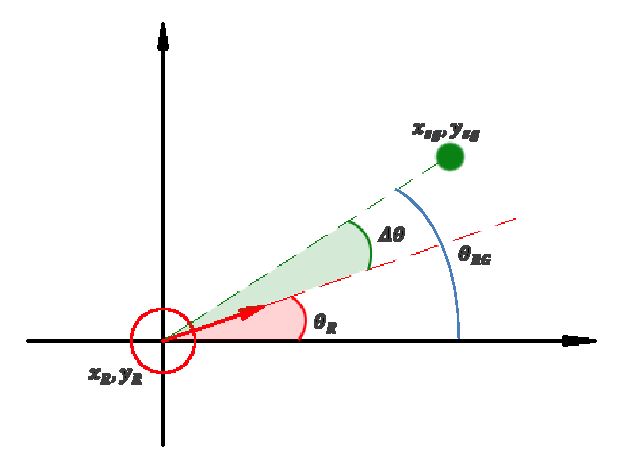
\includegraphics[width=\linewidth]{ex3-coords}
    \caption{Οι θέσεις των σημείων που χρησιμοποιούνται για τον προσδιορισμό των ταχυτήτων. Από~\protect\cite{etsardou-phd}.}\label{fig:ex3-coords}
\end{figure}

Ακολουθείται η διαδικασία που περιγράφεται στην~\cite{etsardou-phd}.
Θεωρούμε ότι τα $x_R$, $y_R$ είναι η αρχή του συστήματος συντεταγμένων και μετασχηματίζουμε τις συντεταγμένες του υποστόχου:
\begin{equation}
    \mathbf{c_{sg}'} = \left(x_{sg}', y_{sg}'\right) = \left(x_{sg} - x_R, y_{sg} - y_R\right)
\end{equation}
και υπολογίζουμε το προσανατολισμό του υποστόχου:
\begin{equation}
    \theta_{sg} = \atantwo{\left(y_{sg}', x_{sg}'\right)}
\end{equation}
Στη συνέχεια, υπολογίζεται ο συντελεστής της γωνιακής ταχύτητας:
\begin{equation}
    \omega = \frac{\Delta{\theta}}{\pi} +
    \begin{cases}
        -2 & \text{Αν $\Delta{\theta} > 0$ και $\Delta{\theta} \geq \pi$} \\
        2  & \text{Αν $\Delta{\theta} < 0$ και $\Delta{\theta} < -\pi$}   \\
        0  & \text{αλλιώς}
    \end{cases}
\end{equation}
ενώ ο συντελεστής της γραμμικής ταχύτητας δίνεται από τη σχέση
\begin{equation}
    u = \left(1-\abs{\omega}\right)^n\label{eq:linear-coeff}
\end{equation}
Η γραμμική ταχύτητα υπολογίζεται έτσι καθώς ο συνδυασμός μεγάλης γραμμικής και γωνιακής ταχύτητας μπορεί να οδηγήσει σε \hyperref[fig:ex3-spiral]{σπειροειδής} κινήσεις του ρομπότ.
Μεγαλύτερες τιμές του $n$ αντιμετωπίζουν πιο ``δραστικά'' το πρόβλημα αλλά μπορεί να οδηγήσουν σε πολύ μικρές γραμμικές ταχύτητες.
Καθώς συναντήσαμε σε μεγάλο βαθμό επιλέξαμε μεγάλη τιμή $n = 6$.
Αυτή η τιμή όμως κάνει το ρομπότ αρκετά αργό και για αυτό το λόγο τροποποιούμε την διαδικασία και επανυπολογίζουμε τον τελικό συντελεστή της γωνιακής ταχύτητας:
\begin{equation}
    \omega' = \sign\left({\omega} \left(1 - u\right)\right)
\end{equation}
Φυσικά, αυτό δεν επηρεάζει τη γραμμική ταχύτητα αλλά κάνει το ρομπότ να στρίβει πιο γρήγορα και να ακολουθεί σχετικά ευθεία τμήματα.

Τέλος οι ταχύτητες υπολογίζονται ως
\begin{equation}
    u_{path} = u \cdot u_{max}
\end{equation}
και
\begin{equation}
    \omega_{path} = \omega \cdot \omega_{max}
\end{equation}

\begin{figure}[htb]
    \centering
    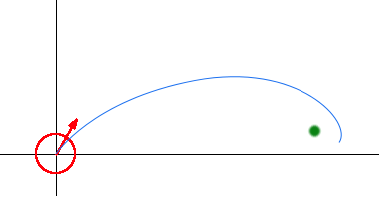
\includegraphics[width=\linewidth]{ex3-spiral}
    \caption{Εκτέλεση σπειροειδούς κίνησης εξαιτίας μεγάλης γραμμικής ταχύτητας. Από~\protect\cite{etsardou-phd}.}\label{fig:ex3-spiral}
\end{figure}

Αποτέλεσμα του path following φαίνεται σε στιγμιότυπο στην εικόνα \ref{fig:random-with-path-following}.

\section{Challenge 4: Ακολούθηση διαδρομής και αποφυγή εμποδίων με τη χρήση αισθητήρων laser}\label{section:ex4}
Σε αυτό το ερώτημα καλούμαστε να συνδυάσουμε τον κώδικα από τα \ref{section:ex1} και \ref{section:ex3} έτσι ώστε το όχημά μας να μπορεί να ακολουθεί ένα δοσμένο target και συγχρόνως να αποφεύγει τα εμπόδια του χάρτη.
Όπως και στο ερώτημα~\ref{section:ex1} χρησιμοποιείται η motor schema στρατηγική από την \cite{etsardou-phd} με τις σχέσεις \ref{eq:u} και \ref{eq:omega}.
Το αρχείο στο οποίο πρέπει να συμπληρωθεί ο κώδικας είναι το
\url{art_autonomous_exploration/src/speeds_assignment.py}.

Ο κώδικας του project τροποποιήθηκε έτσι ώστε αν αποφευχθεί η ύπαρξη των ίδιων υπολογισμών σε δύο σημεία.
Έτσι, η διαφορά  είναι ότι οι συντελεστές \mintinline{python}!linear! και \mintinline{python}!angular! υπολογίζονται με την κλίση της \mintinline{python}!velocitiesToNextSubtarget()!
ενώ στην ενότητα~\ref{section:ex1} ήταν \mintinline{python}!1! και \mintinline{python}!0! αντίστοιχα.

Εδώ, οι συντελεστές $c_u = 0.0001$ και $c_w = 0.0005$ παίρνουν μικρότερη τιμή καθώς θέλουμε να επηρεάζουν λιγότερο τη κίνηση του ρομπότ.
Επίσης, σημειώνεται ότι $c_u < c_w$ καθώς προτιμάμε να έχουμε στροφή του ρομπότ παρά σημαντική μείωση της ταχύτητας του κοντά στα εμπόδια.

Ένα πρόβλημα που συναντήθηκε με αυτό το μοντέλο είναι η πιθανότητα μηδενισμού της ταχύτητας του ρομπότ όταν η ταχύτητες αποφυγής έχουν αντίθετο πρόσημο με τις ταχύτητες από το target.
Όταν οι ταχύτητες παίρνουν πολύ χαμηλές τελικές τιμές το όχημα ακινητοποιείται και δεν υπάρχει τρόπος να αναπτύξει ταχύτητα μέχρι να περάσει το χρονικό όριο και να ανατεθεί νέα διαδρομή.
Μια ευριστική προσέγγιση σε αυτό το πρόβλημα είναι να θέτουμε ταχύτητες στο ρομπότ με τα πρόσημα των ταχυτήτων αποφυγής, έτσι ώστε το ρομπότ να μη ``πέσει'' πάνω σε εμπόδιο και να κουνηθεί από τη θέση του.
Εφόσον ικανοποιηθεί η αρχική συνθήκη (μικρές τελικές ταχύτητες του ρομπότ) εφαρμόζουμε αυτή τη στρατηγική για έναν συνεχόμενο αριθμό επαναλήψεων.
Ο σχετικός κώδικας:
\begin{code}
\caption{Σε περίπτωση μηδενισμού της ταχύτητας θέτουμε νέες ταχύτητες σύμφωνα με τα πρόσημα των ταχυτήτων αποφυγής}
\begin{pythoncode}
if self.stuck_count or (abs(linear) + abs(angular) < (self.MAX_LINEAR_VELOCITY + self.MAX_ANGULAR_VELOCITY) / 2 / 6):
    linear = self.MAX_LINEAR_VELOCITY * np.sign(l_laser) / 2
    angular = self.MAX_ANGULAR_VELOCITY * np.sign(a_laser)
    self.stuck_count = 0 if self.stuck_count >= self.STUCK_LIMIT else self.stuck_count + 1
\end{pythoncode}
\end{code}
Η στρατηγική αυτή παράγει μικτά αποτελέσματα και επιδέχεται βελτίωση.
Θα μπορούσαν για παράδειγμα να συμπεριληφθούν τα δεδομένα από το sonar ώστε να καλύπτονται και τα εμπόδια πίσω από το ρομπότ.

\begin{figure}
    \centering
    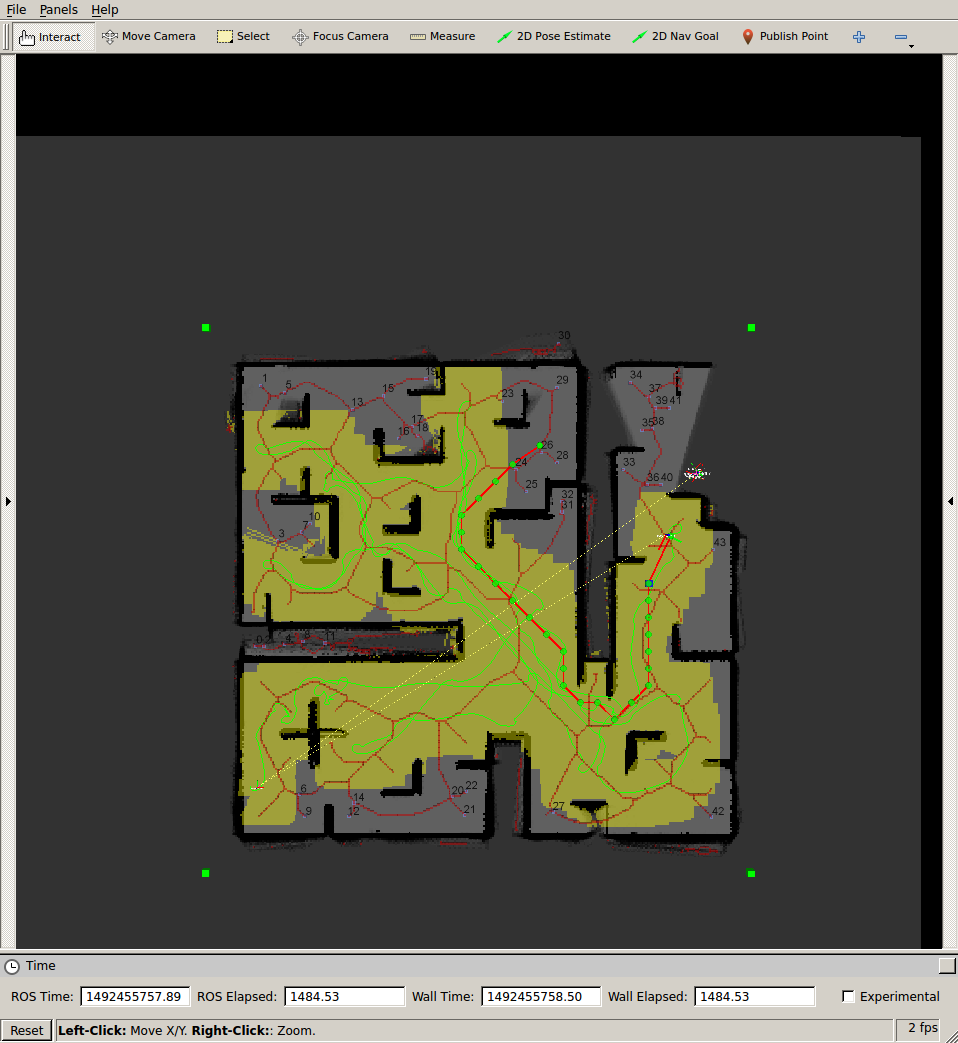
\includegraphics[width=\linewidth]{screens/random-with-path-following}
    \caption{Αποτέλεσμα των Challenge~\hyperref[section:ex3]{3} και~\hyperref[section:ex4]{4}. Path following \& obstacle avoidance με random target selector. Εικόνα από RViz~\protect\cite{rviz}.}
    \label{fig:random-with-path-following}
\end{figure}


%\clearpage
\bibliography{report}
\end{document}
